\documentclass[t,xcolor={svgnames,table}]{beamer}

\mode<presentation>
\usetheme{Warsaw}
\useoutertheme{infolines} 

\usepackage{lmodern}
\usepackage{amsmath}
\usepackage{amsfonts}
\usepackage{bbm}
\usepackage{bm}
\usepackage{nicefrac}
\usepackage{color}
\usepackage{multirow}
\usepackage{multicol}
\usepackage{adjustbox}
\usepackage{tikz}
\usepackage{tikz-dependency}
\usepackage{tikz-qtree}
\usepackage{pgfplots,pgfplotstable}
\usepackage{pgf}
\usepackage{collcell}
\usepackage{booktabs}
\usepackage{soul}
\usepackage{verbatim}

\definecolor{yellow}{rgb}{0.89, 0.61, 0.06}
\definecolor{green}{rgb}{0.0, 0.5, 0.0}
\definecolor{red}{rgb}{0.7, 0.11, 0.11}

% for results matrix
\newcommand{\ApplyGradient}[1]{%
  \pgfmathsetmacro{\PercentColor}{ifthenelse(#1-0 > 0, (#1-21)*.8, 0)}%
  \pgfmathsetmacro{\PercentInverse}{ifthenelse(\PercentColor > 70, 0, 100)}%
  %\textcolor{black!\PercentColor}{#1}
  \edef\x{\noexpand\cellcolor{red!\PercentColor}}\x\textcolor{black!\PercentInverse}{#1}%
}
\newcolumntype{R}{>{\collectcell\ApplyGradient}{c}<{\endcollectcell}}

% Outline slides
\AtBeginSection[]
{\begin{frame} \frametitle{Outline} \tableofcontents[currentsection,currentsubsection] \end{frame}}

\begin{document}


\title[]{The Language of Legal and Illegal Activity \\ on the Darknet}
\author[Daniel Hershcovich]{Leshem Choshen, Dan Eldad, \textbf{Daniel Hershcovich}, \\
Elior Sulem and Omri Abend }
\date[]{ACL 2019 \\
	\hspace{0.5cm}

\includegraphics[width=.5\textwidth]{huji_banner.png}

\includegraphics[width=.1\textwidth]{huji_logo.jpg}}

\begin{frame}
\titlepage
\end{frame}

\section*{Introduction}

{\usebackgroundtemplate{
	\vbox to \paperheight{\vfil\hbox to \paperwidth{\hfil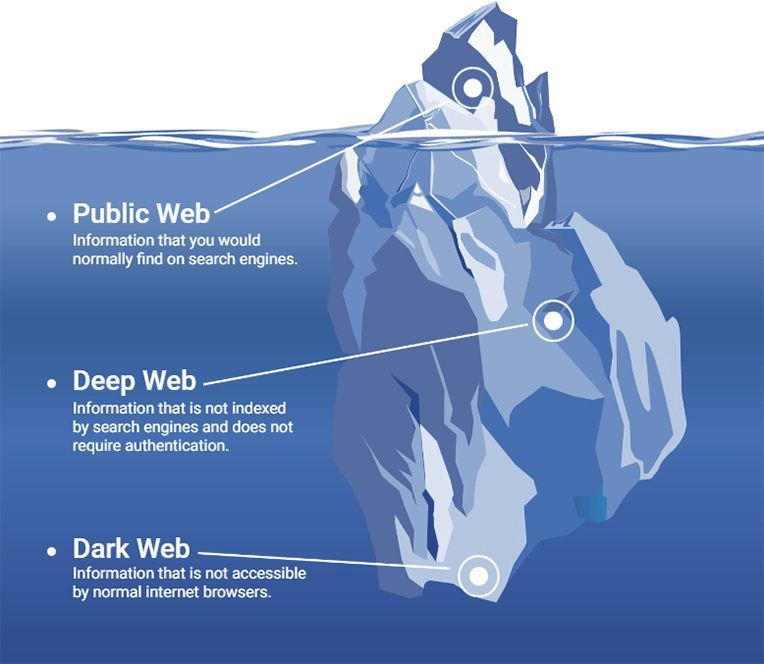
\includegraphics[width=.92\paperwidth]{DarkNet}\hfil}}	
	}%
\begin{frame}
	What is the Dark Web?
	\begin{center}
	\begin{itemize}\setlength\itemsep{1em}
	\item The non-indexed parts of the Internet
	\item Anonymous activities
	\item Both legal and illegal activities
	\end{itemize}
	\end{center}
	% TODO: examples
\end{frame}
}

\begin{frame}
	\frametitle{Darknet}
	
	Used interchangeably in this work:
	\vfill
	
	\begin{minipage}{.6\pagewidth}
	\begin{itemize}\setlength\itemsep{1em}
	\item \textbf{Dark Web}
	\item \textbf{Darknet}
	\item \textbf{Tor} network (Tor: an encrypted browser)
	\item \textbf{Onion} network (.onion top-level domain)
	\end{itemize}
	\end{minipage}
	\begin{minipage}{.3\pagewidth}
	
\includegraphics[width=.3\pagewidth]{Tor.png}
	\end{minipage}
	\vfill
	
	Hosts: \textbf{onion services} (hidden services).
\end{frame}

\begin{frame}
	\frametitle{Darknet Markets}
	
	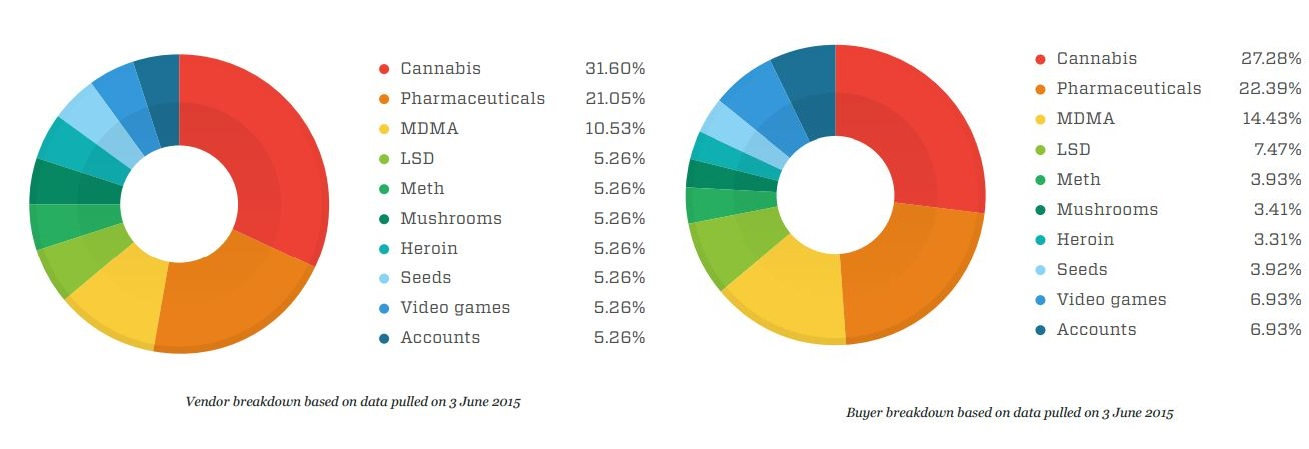
\includegraphics[trim={0 2cm 16cm 1cm},clip,width=\pagewidth]{DeepWeb-Black-markets-vendors-buyers.jpg}\footnote{Paganini (2015). "The Deep Web and Its Darknets".}
\end{frame}

\begin{frame}
	\frametitle{Language of the Darknet}
	
	\begin{center}
	How well do NLP tools work on Darknet text?
	
\includegraphics[width=.4\textwidth]{nlp.png}
	\vfill
	\pause
	
	Can we automatically identify illegal activity?
	
\includegraphics[width=.4\textwidth]{illegal.jpg}
	\end{center}
\end{frame}

\section{Data: Darknet \& eBay}

\begin{frame}
	\frametitle{DUTA-10K}
	
	Dataset of 10367 Onion Services text pages \cite{AlNabki19}.

	\begin{itemize}\setlength\itemsep{1em}
		\item 20\% categorized as illegal and 48\% as legal (32\% unavailable).
		\item Of the illegal (suspicious) websites, 23\% concern illegal \textbf{drugs}.
	\end{itemize}
	\vfill
	\pause

	Distribution of categories:
	
	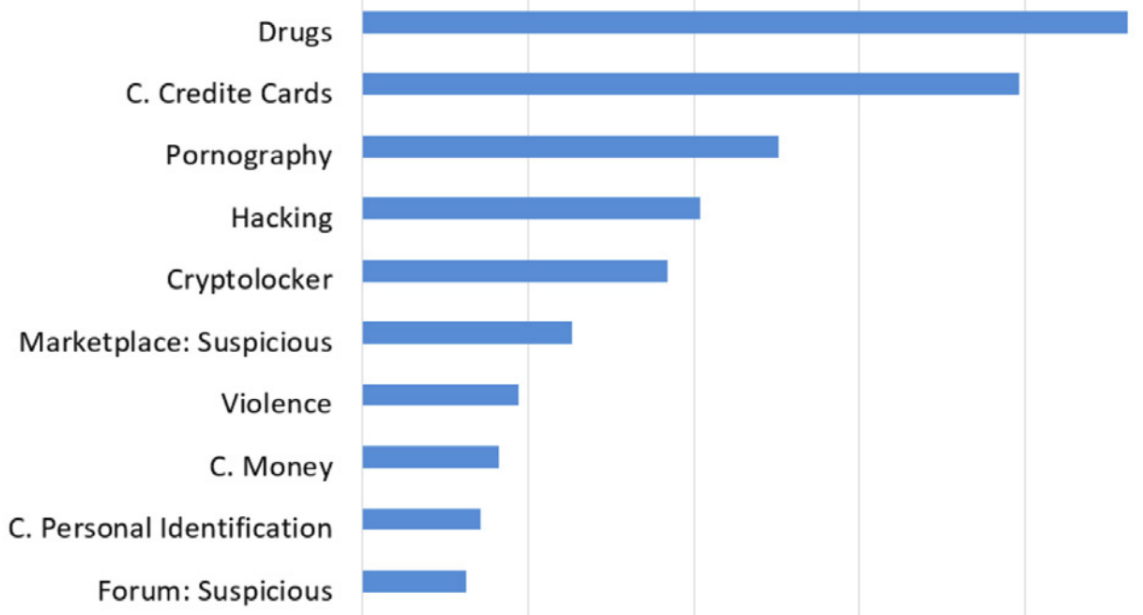
\includegraphics[width=.49\textwidth]{suspicious.png}\hfill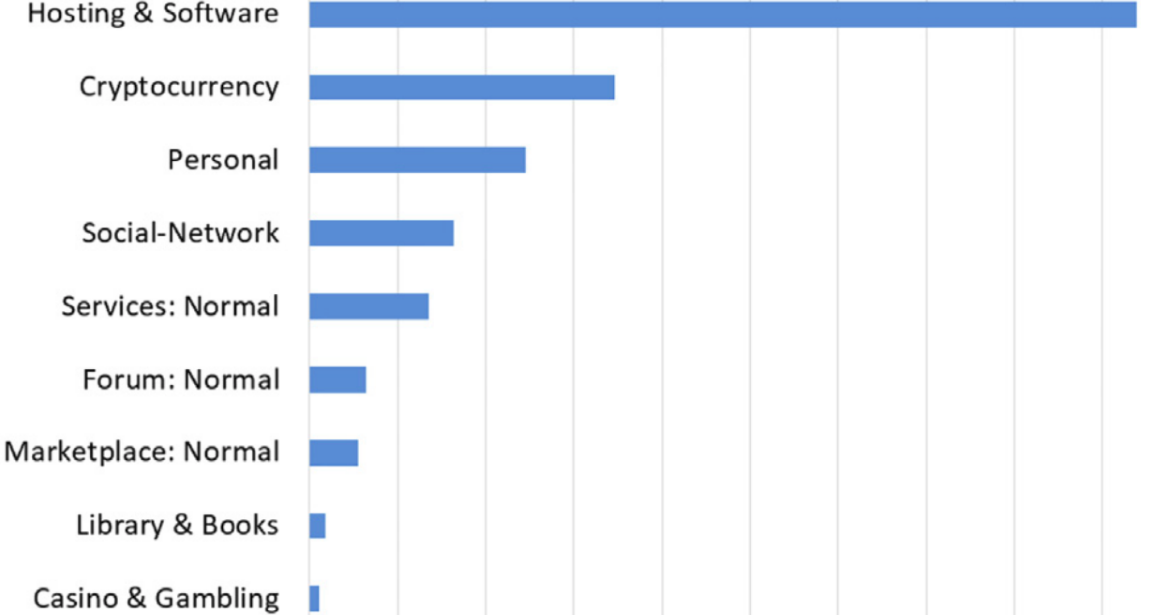
\includegraphics[width=.49\textwidth]{normal.png}
	
	\hspace{2cm} Illegal \hspace{5cm} Legal
\end{frame}

\begin{frame}[fragile]
	\frametitle{Control Data: eBay}
	Product descriptions acquired by searching for drug-related terms.
	\vfill
	
	Do not sell actual drugs, but rather drug-related products.
	\vfill
	
	\begin{center}
	
\includegraphics[width=.5\textwidth]{ebay.png}
	\end{center}
	\vfill
	
\small
\begin{verbatim}
3 Layers  Chip Style Herb Herbal Tobacco Grinder Weed Grinders
Description:
Quantity: 1
Type : Tobacco Crusher
Feature: Stocked,Eco-Friendly
Material: plastic
Size: 42*26mm
Package include:
1PC  Tobacco Crusher
\end{verbatim}
\end{frame}

\begin{frame}
	\frametitle{Data}
	
	\begin{center}
	\def\arraystretch{2}
	\begin{tabular}{c|ccc}
	& Public Web && Dark Web \\ 
	\hline
	\multirow{2}{*}{Legal} & \textbf{\color{yellow} eBay} && \textbf{\color{green} Legal Onion} \\
	& (188 pages, 35,799 words) && (35 pages, 61,655 words) \\\\
	\multirow{2}{*}{Illegal} &&& \textbf{\color{red} Illegal Onion} \\
	&&& (255 pages, 1,438,351 words)
	\end{tabular}
	\end{center}
\end{frame}

\begin{frame}[fragile]
	\frametitle{Cleaning}
	\begin{itemize}\setlength\itemsep{1em}
	%\item Filter out website menu contents, 
	\item Remove non-linguistic content: buttons, encryption keys, metadata, URLs.
	%\vfill
	
	\item Split to paragraphs and join paragraphs to single lines.
	%\vfill
	
	\item Remove duplicate paragraphs.
	%\vfill
	\end{itemize}
	\scriptsize
\begin{verbatim}
	Finest organic cannabis grown by proffessional growers in the
	netherlands.
	We double seal all packages for odor less delivery.
	Shipping within 24 hours!
	              Product                    Price          Quantity
	1g Original Haze                    15 EUR = 0.025 ฿ 1_ X Buy now
	5g Original Haze                    65 EUR = 0.108 ฿ 1_ X Buy now
	1g Bubblegum                        10 EUR = 0.017 ฿ 1_ X Buy now
	5g Bubblegum                        45 EUR = 0.075 ฿ 1_ X Buy now
	1g Jack Herer                       14 EUR = 0.023 ฿ 1_ X Buy now
	5g Jack Herer                       60 EUR = 0.099 ฿ 1_ X Buy now
	1g Chronic                          9 EUR = 0.015 ฿  1_ X Buy now
	5g Chronic                          40 EUR = 0.066 ฿ 1_ X Buy now
	1g Banana Kush                      11 EUR = 0.018 ฿ 1_ X Buy now
\end{verbatim}
\end{frame}

\begin{frame}
	\frametitle{Clean Data}

	Sampled 571 paragraphs from each, for comparable size.
	
	\begin{center}
	\def\arraystretch{2}
	\begin{tabular}{c|ccc}
	& Public Web && Dark Web \\ 
	\hline
	\multirow{2}{*}{Legal} & \textbf{\color{yellow} eBay} && \textbf{\color{green} Legal Onion} \\
	& (14,276 words) && (14,802 words) \\\\
	\multirow{2}{*}{Illegal} &&& \textbf{\color{red} Illegal Onion} \\
	&&& (15,049 words)
	\end{tabular}
	\end{center}
\end{frame}

\section{Domain Differences: Vocabulary \& Named Entities}

\begin{frame}
	\frametitle{Vocabulary}
	Distance between word frequencies distributions, measured by:
	\begin{itemize}
	\item Jensen-Shannon divergence.
	\item L1 distance.
	\end{itemize}
	
	Splitting each dataset in half, we find small ``self-distances'', \\
	but the different domains are about equidistant.
	\vfill
	\pause
	
	\begin{center}
	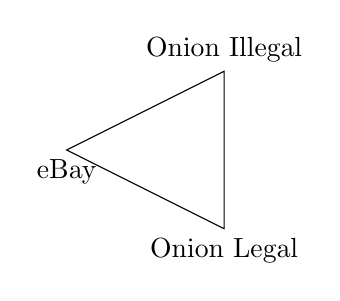
\begin{tikzpicture}
	\draw (0,1) node[anchor=north]{eBay}
	  -- (2,0) node[anchor=north]{Onion Legal}
	  -- (2,2) node[anchor=south]{Onion Illegal}
	  -- cycle;
	\end{tikzpicture}
	\end{center}
	\vfill
	\pause
	
	Legal and illegal Onion should be considered different domains.
\end{frame}

\begin{frame}
	\frametitle{Characteristics of Darknet Data}
	
	Diverse: sub-domains are distinguishable.
	\vfill
	
	Unique: distinguishable from other domains.
	
	\begin{figure}
		\centering
		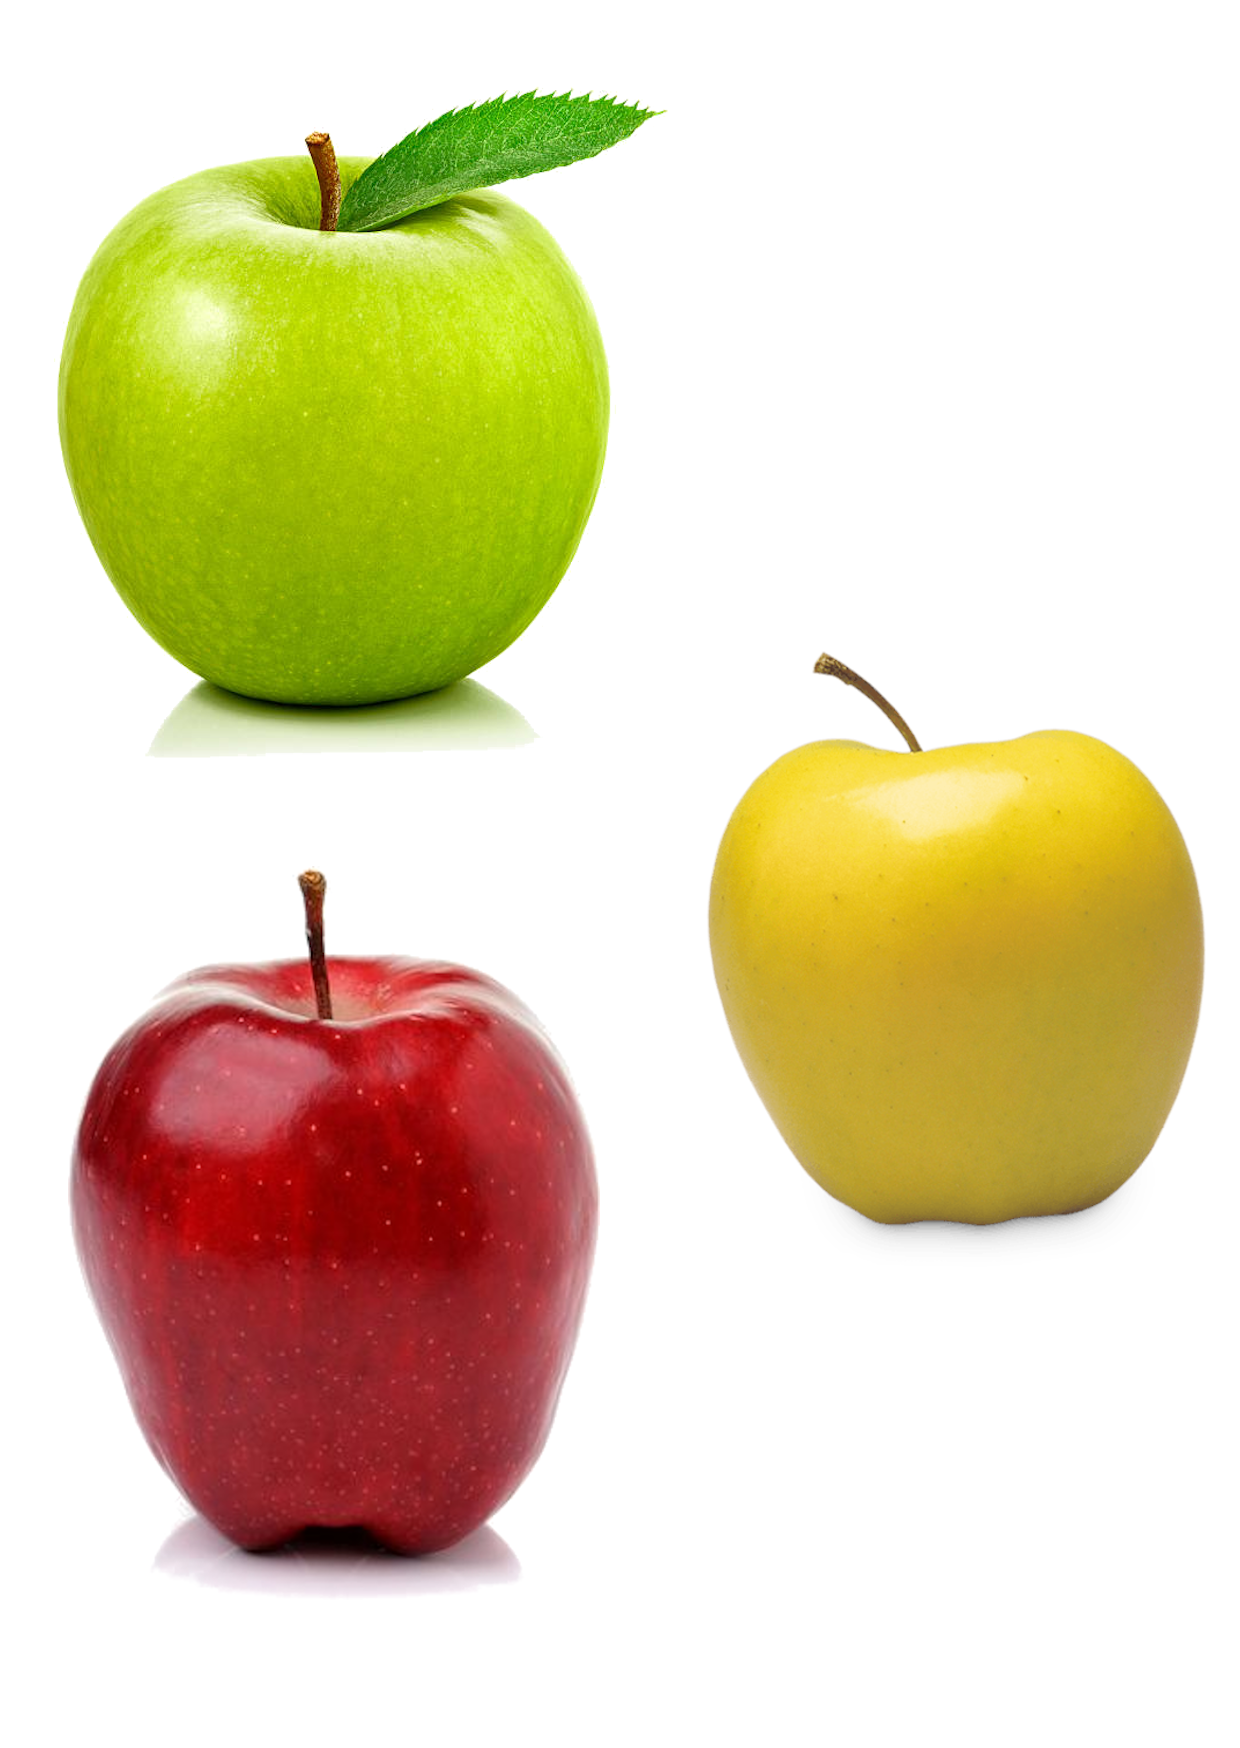
\includegraphics[width=0.3\textwidth]{3different.png}
	\end{figure}
\end{frame}

\begin{frame}
	\frametitle{Named Entities and Wikification}
	
	NE extraction [spaCy] + Wikification \cite{bunescu2006using}.
	\vfill
	
	\begin{center}
	\begin{tabular}{l|r}
	 & \% Wikifiable\\
	 \hline
	eBay & $38.6 \pm2.00$\\
	Illegal Onion & $32.5 \pm1.35$\\
	Legal Onion & $50.8 \pm2.31$
	\end{tabular}
	\end{center}
	\vfill

	By manual inspection, NE precision and recall are low for Illegal Onion.
	
	For example: slang words for drugs (e.g., ``kush'') falsely picked up as NEs.	
	\vfill
	
	$\Rightarrow$ Standard NLP is not suited for this domain.
\end{frame}

\section{Classification: Legal \& Illegal Drugs, eBay}

\begin{frame}
	\frametitle{Classes}
	We identified three domains. Two binary classification settings:
	\begin{center}
	\{ \textbf{\color{yellow} eBay}, \textbf{\color{green} Legal Onion} \}
	\vfill
	
	\{ \textbf{\color{green} Legal Onion}, \textbf{\color{red} Illegal Onion} \}
	\end{center}
	\vfill
	\pause
	
	What are the linguistic features distinguishing them?
	\vfill
	
	\begin{center}
	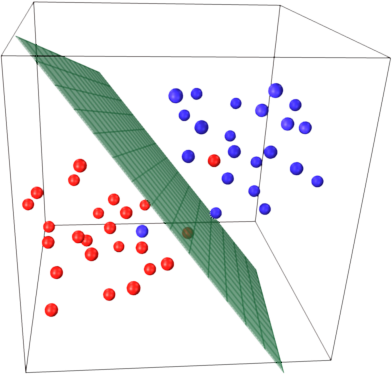
\includegraphics[width=.3\textwidth]{svm.png}
	\end{center}
\end{frame}

\begin{frame}
	\frametitle{Classifiers}
	
	\begin{minipage}{.7\textwidth}
	\begin{itemize}\setlength\itemsep{1em}
		\item NB: Naive Bayes (bag of words)
		\item SVM: Support Vector Machine
		\item BoE: sum/average GloVe + MLP
		\item seq2vec: BiLSTM + MLP
		\item attention: ELMo + BCN (self-attention)
	\end{itemize}
	\end{minipage}
	\begin{minipage}{.29\textwidth}
	\centering
	\hspace{-2cm}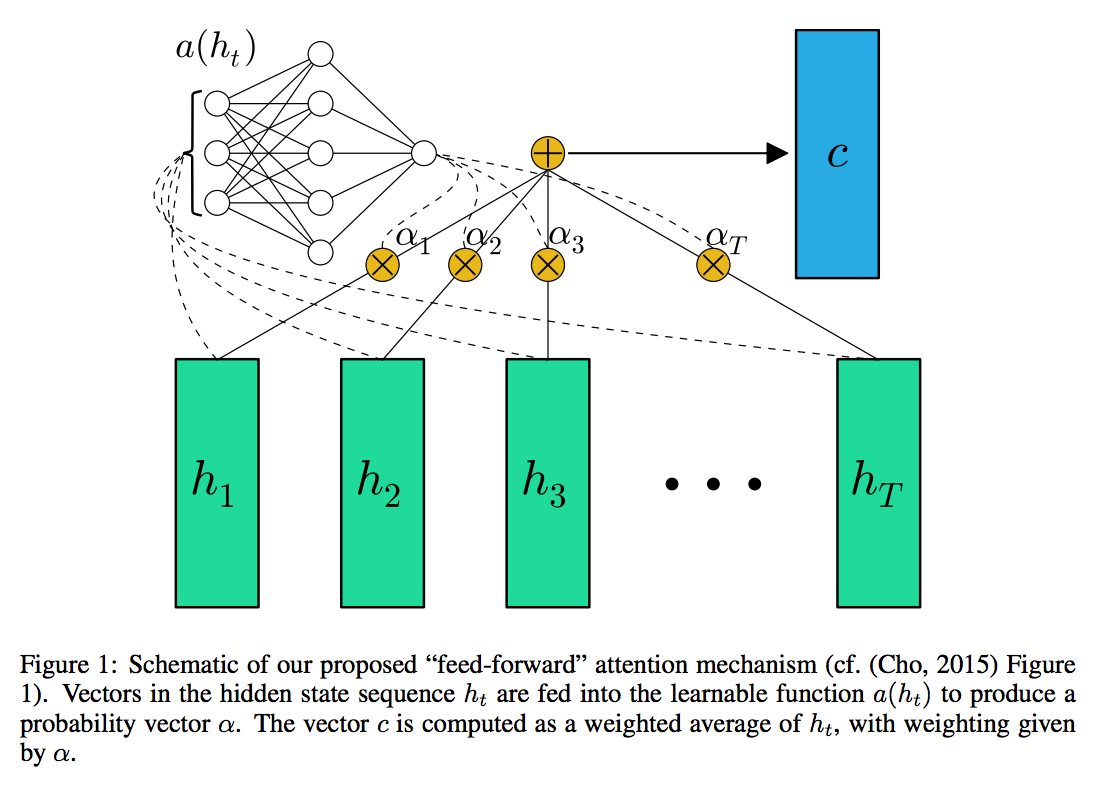
\includegraphics[trim={3cm 3cm 3cm 0},clip,width=1.5\textwidth]{FeedForwardAttention.png}
	
	
\includegraphics[width=.7\textwidth]{elmo.jpg}
	\end{minipage}
\end{frame}

\begin{frame}
	\frametitle{Manipulations}
	
	\begin{itemize}\setlength\itemsep{1em}
	    \item Full original text
	\end{itemize}
	\vfill
	
	\begin{minipage}{.35\textwidth}
	\begin{itemize}\setlength\itemsep{1em}
		\item Drop \textbf{content} words
		\item Drop \textbf{function} words
	\end{itemize}
	\end{minipage}
	\begin{minipage}{.59\textwidth}
	\begin{itemize}\setlength\itemsep{1em}
		\item Replace \textbf{content} words with their POS
		\item Replace \textbf{function} words with their POS
	\end{itemize}
	\end{minipage}
	\vfill
	
    \[\{\textsc{adj, adv, noun, propn, verb, x, num}\}\]
	\vfill
	\pause
	
	{\color{green}
	\setlength{\tabcolsep}{2.3pt}
	\begin{tabular}{ccccccccccc}
	Generic&Viagra&(&Oral&Jelly&)&is&used&for&Erectile&Dysfunction\\
	\small\textsc{propn} & \small\textsc{propn} &(& \small\textsc{propn} & \small\textsc{propn} &)& \small\textsc{verb} & \small\textsc{verb} & for & \small\textsc{propn} & \small\textsc{propn}
	\end{tabular}}
	\vfill
	\pause
	
	{\color{red}
	\setlength{\tabcolsep}{9.5pt}
	\begin{tabular}{ccccccc}
	Welcome&to&SnowKings&Good&Quality&Cocaine&!\\
	\small\textsc{verb} & to & \small\textsc{propn} & \small\textsc{propn} & \small\textsc{propn} & \small\textsc{propn} & !
	\end{tabular}}
\end{frame}

\begin{frame}
	\frametitle{Results: eBay vs. Legal Onion Drugs}
	
	Clear separation by content (by NB), but also by function (by SVM).
	
	\begin{center}
		\setlength{\tabcolsep}{8pt}\def\arraystretch{1.8}
		\begin{tabular}{l *{5}{R}}
		& \multicolumn{1}{c}{\bf \rotatebox{90}{full}}
		& \multicolumn{1}{c}{\bf \rotatebox{90}{drop}\rotatebox{90}{content}}
		& \multicolumn{1}{c}{\bf \rotatebox{90}{drop}\rotatebox{90}{function}}
		& \multicolumn{1}{c}{\bf \rotatebox{90}{pos}\rotatebox{90}{content}}
		& \multicolumn{1}{c}{\bf \rotatebox{90}{pos}\rotatebox{90}{function}}\\
		\hline
		NB & 91.4 & 57.8 & 90.5 & 56.9 & 92.2\\
		SVM & 63.8 & 64.7 & 63.8 & 68.1 & 63.8\\
		BoE$_\mathrm{sum}$ & 66.4 & 56.0 & 63.8 & 50.9 & 76.7\\
		BoE$_\mathrm{average}$ & 75.0 & 55.2 & 59.5 & 50.0 & 75.0\\
		seq2vec & 73.3 & 53.8 & 65.5 & 65.5 & 75.0\\
		attention & 82.8 & 57.5 & 85.3 & 62.1 & 82.8
		\end{tabular}
	\end{center}
\end{frame}

\begin{frame}
	\frametitle{Results: Legal vs. Illegal Onion Drugs}
	
	Harder to distinguish by content, easier by POS distribution (SVM again).
	
	\begin{center}
		\setlength{\tabcolsep}{8pt}\def\arraystretch{1.8}
		\begin{tabular}{l *{5}{R}}
		& \multicolumn{1}{c}{\bf \rotatebox{90}{full}}
		& \multicolumn{1}{c}{\bf \rotatebox{90}{drop}\rotatebox{90}{content}}
		& \multicolumn{1}{c}{\bf \rotatebox{90}{drop}\rotatebox{90}{function}}
		& \multicolumn{1}{c}{\bf \rotatebox{90}{pos}\rotatebox{90}{content}}
		& \multicolumn{1}{c}{\bf \rotatebox{90}{pos}\rotatebox{90}{function}}\\
		\hline
		NB & 77.6 & 53.4 & 87.9 & 51.7 & 77.6\\
		SVM & 63.8 & 66.4 & 63.8 & 70.7 & 63.8\\
		BoE$_\mathrm{sum}$ & 52.6 & 61.2 & 74.1 & 50.9 & 51.7\\
		BoE$_\mathrm{average}$ & 57.8 & 57.8 & 52.6 & 55.2 & 50.9\\
		seq2vec & 56.9 & 55.0 & 54.3 & 59.5 & 49.1\\
		attention & 64.7 & 51.4 & 62.9 & 55.2 & 69.0
		\end{tabular}
	\end{center}
\end{frame}

\begin{frame}
	\frametitle{Classification Challenges}
	
	Simple classifiers (NB, SVM) work best.
	\begin{itemize}\setlength\itemsep{1em}
	\item Small training data.
	\item Non-standard language.
	\item Understudied domain.
	\end{itemize}
\end{frame}

\section{Cross-Domain Classification: Legal \& Illegal Forums}

\begin{frame}
	\frametitle{Darknet Forums}
	
	Can we generalize beyond drugs?
	\vfill
	\pause
	
	DUTA-10K also contain
	{\color{green}Legal Forums} and {\color{red}Illegal Forums}.
	
	Multi-topic and user-generated.
	\vfill
	
	\begin{center}
	
\includegraphics[width=.5\textwidth]{forum.jpg}
	\end{center}
\end{frame}

\begin{frame}
	\frametitle{Results: Legal vs. Illegal Onion Forums}
	
	Harder for most classifiers, but SVM succeeds using content and function.
	
	\begin{center}
		\setlength{\tabcolsep}{8pt}\def\arraystretch{1.8}
		\begin{tabular}{l *{5}{R}}
		& \multicolumn{1}{c}{\bf \rotatebox{90}{full}}
		& \multicolumn{1}{c}{\bf \rotatebox{90}{drop}\rotatebox{90}{content}}
		& \multicolumn{1}{c}{\bf \rotatebox{90}{drop}\rotatebox{90}{function}}
		& \multicolumn{1}{c}{\bf \rotatebox{90}{pos}\rotatebox{90}{content}}
		& \multicolumn{1}{c}{\bf \rotatebox{90}{pos}\rotatebox{90}{function}}\\
		\hline
		NB & 74.1 & 50.9 & 78.4 & 50.9 & 72.4\\
		SVM & 85.3 & 75.9 & 56.0 & 81.9 & 81.0\\
		BoE$_\mathrm{sum}$ & 25.9 & 32.8 & 21.6 & 36.2 & 35.3\\
		BoE$_\mathrm{average}$ & 40.5 & 42.2 & 31.9 & 48.3 & 53.4\\
		seq2vec & 50.0 & 48.9 & 50.9 & 28.4 & 51.7\\
		attention & 31.0 & 37.2 & 33.6 & 27.6 & 30.2
		\end{tabular}
	\end{center}
\end{frame}

\begin{frame}
	\frametitle{Results: Trained on Drugs, Tested on Forums}
	
	Effective cross-domain generalization even with bag-of-words.
	
	\begin{center}
		\setlength{\tabcolsep}{8pt}\def\arraystretch{1.8}
		\begin{tabular}{l *{5}{R}}
		& \multicolumn{1}{c}{\bf \rotatebox{90}{full}}
		& \multicolumn{1}{c}{\bf \rotatebox{90}{drop}\rotatebox{90}{content}}
		& \multicolumn{1}{c}{\bf \rotatebox{90}{drop}\rotatebox{90}{function}}
		& \multicolumn{1}{c}{\bf \rotatebox{90}{pos}\rotatebox{90}{content}}
		& \multicolumn{1}{c}{\bf \rotatebox{90}{pos}\rotatebox{90}{function}}\\
		\hline
		NB & 78.4 & 63.8 & 89.7 & 63.8 & 79.3\\
		SVM & 62.1 & 69.0 & 54.3 & 69.8 & 62.1\\
		BoE$_\mathrm{sum}$ & 45.7 & 50.9 & 49.1 & 50.9 & 50.0\\
		BoE$_\mathrm{average}$ & 49.1 & 51.7 & 51.7 & 52.6 & 58.6\\
		seq2vec & 51.7 & 61.1 & 51.7 & 54.3 & 57.8\\
		attention & 65.5 & 59.2 & 65.5 & 50.9 & 66.4
		\end{tabular}
	\end{center}
\end{frame}

\section*{}

\begin{frame}
	\frametitle{Conclusion}
	Differences between legal and illegal Darknet sites:	
	\begin{itemize}\setlength\itemsep{1em}
	\item Vocabulary
	\item Shallow syntax (POS)
	\item Named entities
	\end{itemize}
	\vfill
	\pause
	
	Identified by:
	\begin{itemize}\setlength\itemsep{1em}
	\item Word statistics: diverse and unique
	\item Wikification: works less well on illegal
	\item Predictive: simple classifiers work best
	\end{itemize}
	\vfill
	\pause
	
	\begin{minipage}{.7\textwidth}
	Code: {\color{blue}\url{https://github.com/huji-nlp/cyber}}
	
	Data: {\color{blue}\url{dan.eldad1@mail.huji.ac.il}}
	\end{minipage}
	\pause
	\begin{minipage}{.28\textwidth}
	\centering\vspace{-2cm}
	
\includegraphics[width=.8\textwidth]{onion.jpg}
	
	Thanks!
	\end{minipage}
\end{frame}

\begin{frame}[allowframebreaks]
\frametitle{References}
\bibliographystyle{apalike}
\tiny\bibliography{acl2019}
\end{frame}

\end{document}
